\chapter{Grundlagen}
\section{Bildkompression}
Für die Anwendung der \acl{ELA} zu verstehen, ist es wichtig die Grundlagen der Bildkompression zu kennen. Die \ac{ELA} setzt an den Eigenschaften an, welche Bilder in Verlustbehafteten Bildformaten aufweisen.\\
Eines der bekanntesten Bildformate welches diese Eigenschaft ausweist ist JPEG, eine Norm (ISO/IEC 10918-1 oder CCITT T.81) zur Bildkomprimierung welche von der \ac{JPEG} entwickelt wurde. Das \ac{JPEG}-Schema ist zwar bei genauer Betrachtung recht komplex, das Grundprinzip ist allerdings leicht zu verstehen.\\
In einem ersten Schritt wird das Bitmap-Bild in 8x8 Matrizen aufgeteilt und mit Hilfe der \acp{DCT} von einer 8x8 Ortsmatrix, in eine 8x8 Frequenzmatrix umgewandelt. Alle folgenden Schritte arbeiten nun mit der diesen Matrizen, das Bild wird nicht mehr als ganzes betrachtet.\\
Jede dieser Pixelgruppen wird separat mit einer eigenen DCT kodiert und kann auch wieder verlustfrei reproduziert werden. Abbildung \ref{fig:Dctjpeg} zeigt die Basisfunktion einer zweidimensionalen DCT (Quantisierungstabelle) wobei zu sehen ist, dass die Frequenz von links nach rechts und von oben nach unten zunimmt. Bei der anschließenden Quantisierung werden die höherfrequenten Anteile des Bildes geringer gewichtet, als die niederfrequenten und die Koeffizienten welche nahezu 0 sind werden auf 0 gesetzt.\cite{Zichner2002}
Der letzte Schritt der Kompression ist die Entropie-Kodierung der Koeffizienten, wobei hier meistens die Huffman-Kodierung zum Einsatz kommt.\\
Die Dateigröße des komprimierten Bildes hängt vom Inhalt und der Qualität des Originalbildes ab. In der Regel benötigt ein Bild mit wenig Details wie zum Beispiel einem Foto des blauen Himmels weniger Speicherplatz als ein Bild welches viele Details enthält wie z.B. ein Foto einer Menschenmenge.\cite{Warif_2015}\\

\begin{figure}[H]
	\begin{center}
		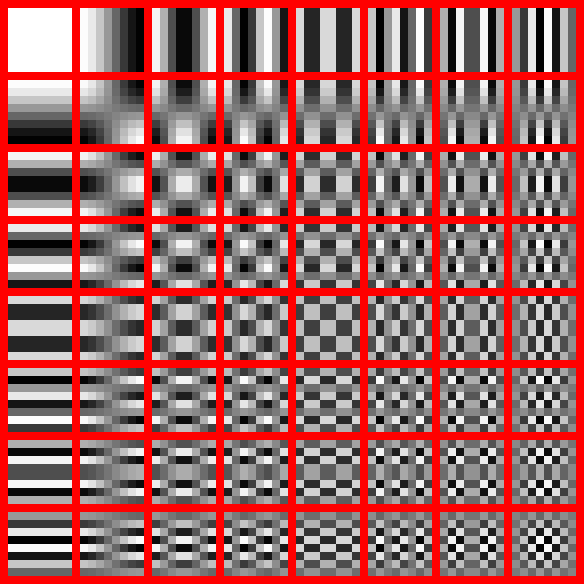
\includegraphics[scale=0.4]{images/Dctjpeg.png}
		\caption{Basisfunktion einer zweidimensionalen DCT (Quantisierungstabelle)}
		\label{fig:Dctjpeg}
	\end{center}
\end{figure}

\section{Erkennung von Kompressionsartefakten}
In den meisten Fällen einer Bildmanipulation wird ein Bild neu komprimiert, speziell dann wenn es durch die Bildbearbeitungssoftware abgespeichert wird. Dieser Vorgang verändert die ursprüngliche Komprimierungseigenschaften, das Ziel besteht nun darin diese Komprimierungseigenschaften, auch Artefakte genannt, zu analysieren und innerhalb eines Bildes möglicherweise Inkonsistenzen zu erkennen.\\
Hier gibt es zwei methodische Vorgehensweisen um solche Artefakte zu unterscheiden. Erstere Methode versucht Inkonsistenzen in der JPEG-Quantisierungstabellen zu erkennen, zweitere verwendet die Komprimierungsartefakte im Frequenzbereich des Bildes um so eine Signatur zu bilden und zwischen unterschiedlichen Kompressionscharakteristika zu unterscheiden.\cite{Chen2011} In folgenden Unterpunkten werden beide Ansätze nochmals kurz zusammengefasst:

\subsection{Inkonsistenz bei der Quantisierungstabelle}
Beim kodieren eines JPEG Bildes werden alle 8x8 Blöcke bei der Entropie-Kodierung durch dieselbe Quantisierungstabelle kodiert. Wenn nun ein Manipuliertes Bild vorliegt können Bereiche dessen, Eigenschaften von verschiedenen Quantisierungstabellen enthalten was zu einer Inkonsistenz führt. Zur Schätzung der Quantisierungstabelle des Originalbildes bei JPEG gibt es mehrere mathematische Verfahren welche anwendbar sind: Gängig ist unter anderem die Maximum-Likelihood-Schätzung auch als \emph{Methode der größten Plausibilität} bezeichnet oder die Maximum-a-posteriori-Schätzung.\cite{Chen2011} Auf die mathematischen Schätzverfahren wird nicht weiter Bezug genommen.\\
Mit der geschätzten Quantisierungstabelle ist es nun möglich, Blockinkonsistenzen zu erkennen und die Blöcke welche von einer Bildmanipulation betroffen sind zu lokalisieren. Die Möglichkeit, dass die Schätzung stark von der verwendeten Quantisierungstabelle des Originalbildes abweicht erhöht sich aber mit jeder erneuten Kompression des Manipulierten Bildes.\\
In der Praxis findet eine erneute Kompression einer Manipulation meist nicht durch den Ersteller sondern durch das verwendete Medium statt. So werden in den allermeisten sozialen Netzwerken Bilder nach dem Hochladen erneut komprimiert um die Dateigröße zu verringern und so Zeit beim erneuten Abruf über das Netzwerk zu sparen. Auch die gängigen Messenger-Dienste komprimieren das Bild vor dem Absenden. Eine bessere Erkennung von mehrfach komprimierten Bildern liefert die Methode welche im nächsten Unterpunkt beschrieben wird.



\subsection{Anomalie von Kompressionsartefakten}